\subsection{Components}

\note{Feel free to move and change the name of this subsection later}

This is my cool document. I have a lot of cool things to say. I was here. \note{note to self: Improve this introduction}


\begin{figure*}
    \begin{center}
    \begin{tikzpicture}[auto, node distance=2cm,>=latex']
        
        % Inputs
        % \node [input] (input_name) {};
        \node [input] (SDI12_sensor_1) {};
        \node [input, yshift= 1cm] (SDI12_sensor_2) {};
        \node [input, yshift= -1cm, xshift= -1cm] (analogue_input) {};

        % Blocks
        % \node [block, location, node distance=xcm, minimum width=xcm] (block_name) {label};
        \node [block, right of=SDI12_sensor_1, node distance=3cm, minimum width=2cm, minimum height=3cm] (RP2040) {RP2040};
        \node [block, left of=RP2040, yshift= -1cm, node distance=2cm, minimum width=1cm, minimum height=1cm] (ADC) {ADC};
        \node [block, right of=RP2040, node distance=2cm, minimum width=1cm, minimum height=1cm] (DAC) {DAC};

        % Outputs
        % \node [output, location] (output_name) {};
        \node [output, right of=DAC] (dew_point_generator) {};

        % Arrows
        % \draw [->] (point_A) -- node {label} (point_B);
        \draw [->] (SDI12_sensor_1) -- ++ (2,0) node [near start, above] {SDI-12 sensor 1} (RP2040);
        \draw [->] (SDI12_sensor_2) -- ++ (2,0) node [near start, above] {SDI-12 sensor 2} (RP2040);
        \draw [->] (ADC) -- ++ (1,0) node [near start, above] {} (RP2040);

        \draw [->] (RP2040) -- (DAC);
        \draw [->] (DAC) -- node [near end, above] {Dew Point Generator} (dew_point_generator);
        \draw [->] (analogue_input) -- node [near start, above] {Analogue input} (ADC);

    \end{tikzpicture}
    \end{center}
    \caption{Block of diagram of the system}
    \label{block_diagram}
\end{figure*}

As seen in \cref{block_diagram} there were lots of blocks


Sensors

SDI-12

\begin{figure}
    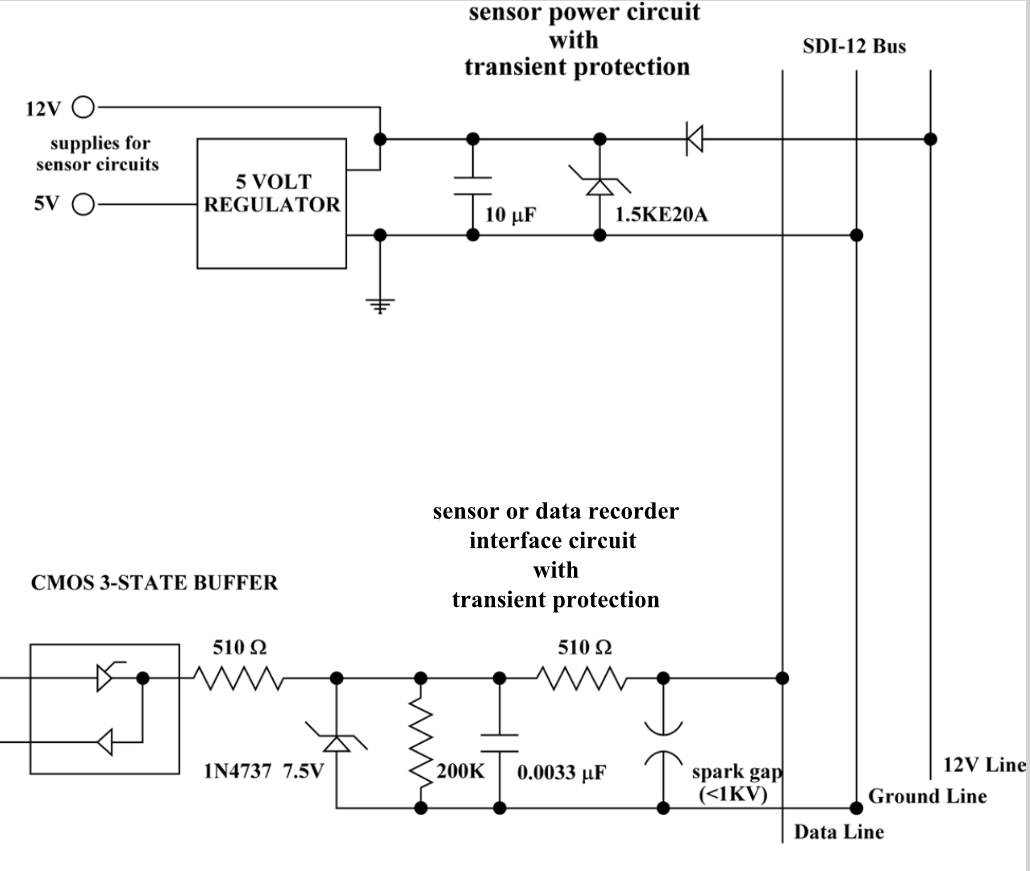
\includegraphics[width=\linewidth]{figures/SDI-12 circuit.png}
    \caption{SDI-12 Circuit Diagram from \cite{sdi12_datasheet}}
    \label{sdi12_circuit}
\end{figure}

Load Cell (MT603)
analogue signal, therefore requires ADC?

Sap Flow Sensor (SF5)
uses SDI-12

Leaf thermistor
uses SDI-12

Things to Consider:
- crystal like in assignment 1?
- ADC for load cell?
- Interface for DAC?